\subsection{MC validation}

\begin{itemize}
	\item A monte carlo sample of QCD (with pythia) and \ttbar were also used to test the 4b SR before unblinding. 
\end{itemize}

\textbf{Validate with data trained networks}

%\begin{table}[ht]
%    \centering
%    \caption{The 4b and reweighted 2b yields in QCD and \ttbar MC simulation in SR. The errors on the background prediction include the 2b Poisson statistic error, bootstrap error and shape systematic error.}
%    \setlength\extrarowheight{5pt}
%    \begin{tabular}{cccc}
%        \toprule
%            Year & 4b Yield & Background Prediction & Deviation ($\sigma$) \\
%        \midrule
%            2016 & 3312.6 $\pm$ 227.3 & 2997.2 $\pm$ 208.8 & 1.02 \\
%            2017 & 4835.1 $\pm$ 270.5 & 4551.7 $\pm$ 295.8 & 0.71 \\
%            2018 & 8018.3 $\pm$ 435.3 & 7321.2 $\pm$ 473.5 & 1.08 \\
%        \bottomrule
%    \end{tabular}
%    \label{tbl:mc-4b-yields}
%\end{table}

\begin{figure}[ht]
    \centering
    \subfloat[$m_{\higgs\higgs}$ in 2016]{
    	\label{fig:mhh-4b-2016-mc-bkg}%
        \includegraphics[width=0.33\textwidth]{\figpath/mc-validation/bkgd-4b-nocat/MAY21-Qs45-MeanWeight-MC-m-hh-Signal-Region-NN-16-4binclusive.png}
    }
    \subfloat[$m_{\higgs\higgs}$ in 2017]{
    	\label{fig:mhh-4b-2017-mc-bkg}%
        \includegraphics[width=0.33\textwidth]{\figpath/mc-validation/bkgd-4b-nocat/MAY21-Qs45-MeanWeight-MC-m-hh-Signal-Region-NN-17-4binclusive.png}
    }
    \subfloat[$m_{\higgs\higgs}$ in 2018]{\label{fig:mhh-4b-2018-mc-bkg}%
            \includegraphics[width=0.33\textwidth]{\figpath/mc-validation/bkgd-4b-nocat/MAY21-Qs45-MeanWeight-MC-m-hh-Signal-Region-NN-18-4binclusive.png}
    }
    \caption{$m_{\higgs\higgs}$ \textbf{data reweighted} 2b events and 4b events \textbf{evaluated on the QCD and \ttbar \ MC} samples. 
             The background estimate error includes the 2b poisson, deep ensembles, and CR1/CR2 shape systematic errors.}
    \label{fig:bkgd4b-mc-bkg}
\end{figure}



\textbf{Validate with MC (re)trained networks}

\def\figpath{figures/nr-int-note/appendices/bkgd-mc-validation/V2}

\begin{figure}[ht]
    \centering
    \subfloat[$m_{\higgs\higgs}$ in 2016]{\label{fig:mhh-4b-2016-mcweight-bkg}%
            \includegraphics[width=0.33\textwidth]{\figpath/mc-weights/bkgd-4b-nocat/sig/2016/MAY21-Qs45-MeanWeight-MC-m-hh-Signal-Region-NN-16-4binclusive.png}
    }
    \subfloat[$m_{\higgs\higgs}$ in 2017]{\label{fig:mhh-4b-2017-mcweight-bkg}%
            \includegraphics[width=0.33\textwidth]{\figpath/mc-weights/bkgd-4b-nocat/sig/2017/MAY21-Qs45-MeanWeight-MC-m-hh-Signal-Region-NN-17-4binclusive.png}
    }
    \subfloat[$m_{\higgs\higgs}$ in 2018]{
    	\label{fig:mhh-4b-2018-mcweight-bkg}%
         \includegraphics[width=0.33\textwidth]{\figpath/mc-weights/bkgd-4b-nocat/sig/2018/MAY21-Qs45-MeanWeight-MC-m-hh-Signal-Region-NN-18-4binclusive.png}
    }
    \caption{$m_{\higgs\higgs}$ \textbf{MC reweighted} 2b events and 4b events evaluated on the QCD and \ttbar \ MC samples. 
             The background estimate error includes the 2b poisson, deep ensembles, and CR1/CR2 shape systematic errors.}
    \label{fig:bkgd4b-mcweight-bkg}
\end{figure}

%\begin{table}[ht]
%    \centering
%    \caption{\label{tbl:mcweight-4b-yields} 4b yield and reweighted 2b yield of 
%             QCD and \ttbar MC samples in SR. MC derived weights are used. 
%             The error of background prediction includes 2b poisson statistic 
%             error, bootstrap error and shape systematic error.}
%    \setlength\extrarowheight{5pt}
%    \begin{tabular}{cccc}
%        \toprule
%            year & 4b yield & background prediction & deviation \\
%        \midrule
%            2016 & 3312.6 $\pm$ 227.3 & 2949.4 $\pm$ 233.0 & 1.12 \\
%            2017 & 4835.1 $\pm$ 270.5 & 4746.5 $\pm$ 301.2 & 0.22 \\
%            2018 & 8018.3 $\pm$ 435.3 & 7628.3 $\pm$ 518.9 & 0.58 \\
%        \bottomrule
%    \end{tabular}
%\end{table}




